\section{Admin-Page}
\label{adminpage}


Ist der Benutzer als Admin angemeldet erscheint unter dem Vorschlag erstellen Knopf ein 
\textit{Vorschlagsverwaltung/Park hinzufügen}, welcher einen auf die \textit{Recommendation-View}
weiterleitet. 


\subsection{Recommendation-View}

\begin{figure}[H]
    \begin{center}
      \frame{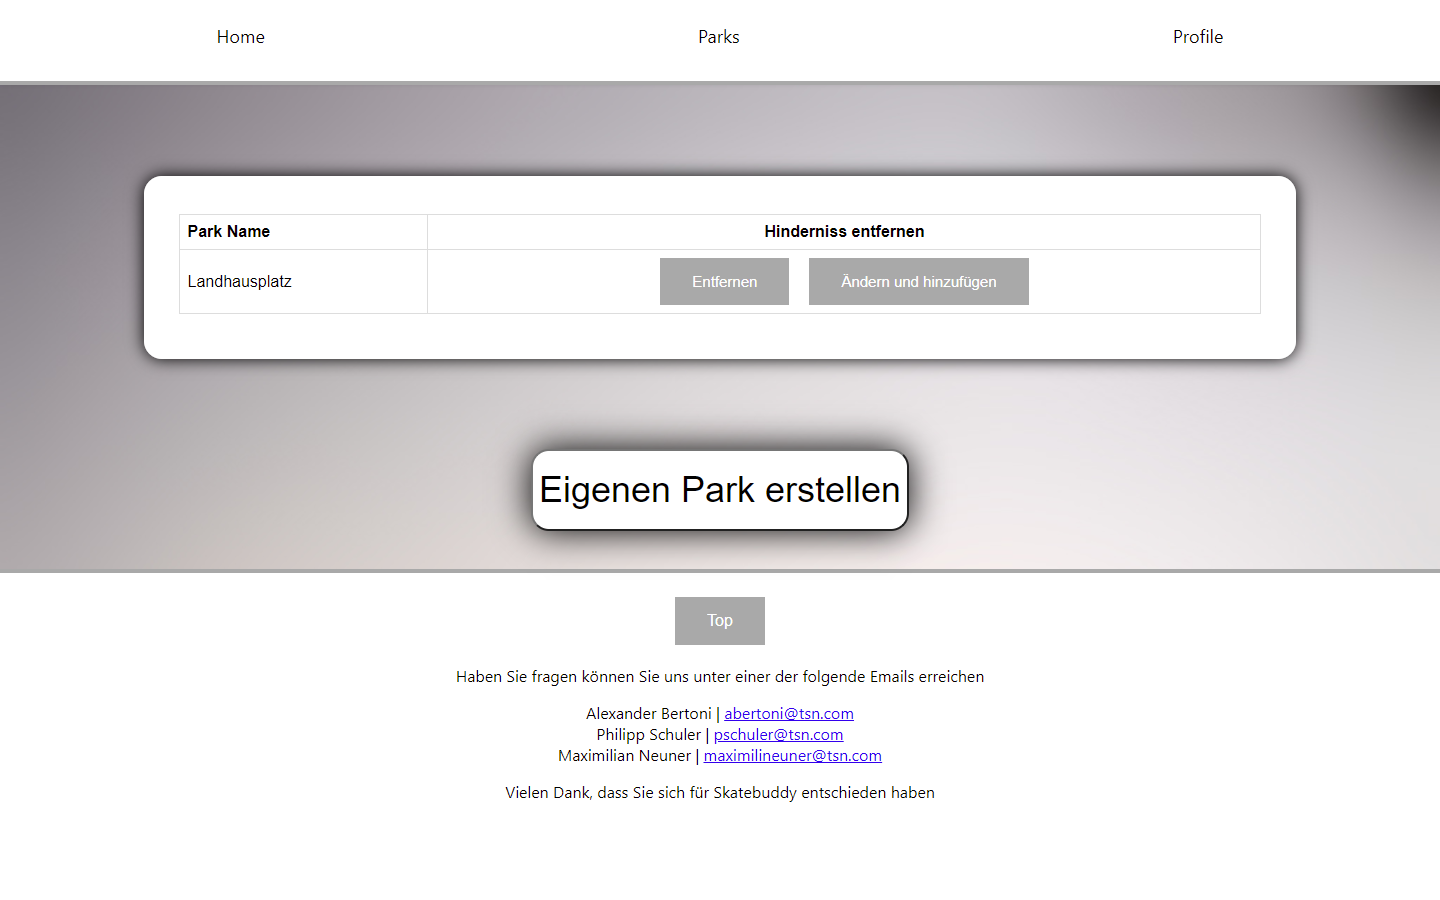
\includegraphics[width=1\textwidth]{Website/Recoom.png}}
      \caption{Liste der Vorschläge}
    \end{center}
\end{figure}

In dieser Ansicht kann der Admin alle erstellen Vorschläger der User erstellen. Er kann sie von hier 
aus löschen oder bearbeiten und als Park hinzufügen. Er kann von hier aus auch selbst einen komplett neuen
Park hinzufügen, ohne einen Vorschlag zu bearbeiten.

\subsection{Park hinzufügen}

\begin{figure}[H]
    \begin{center}
      \frame{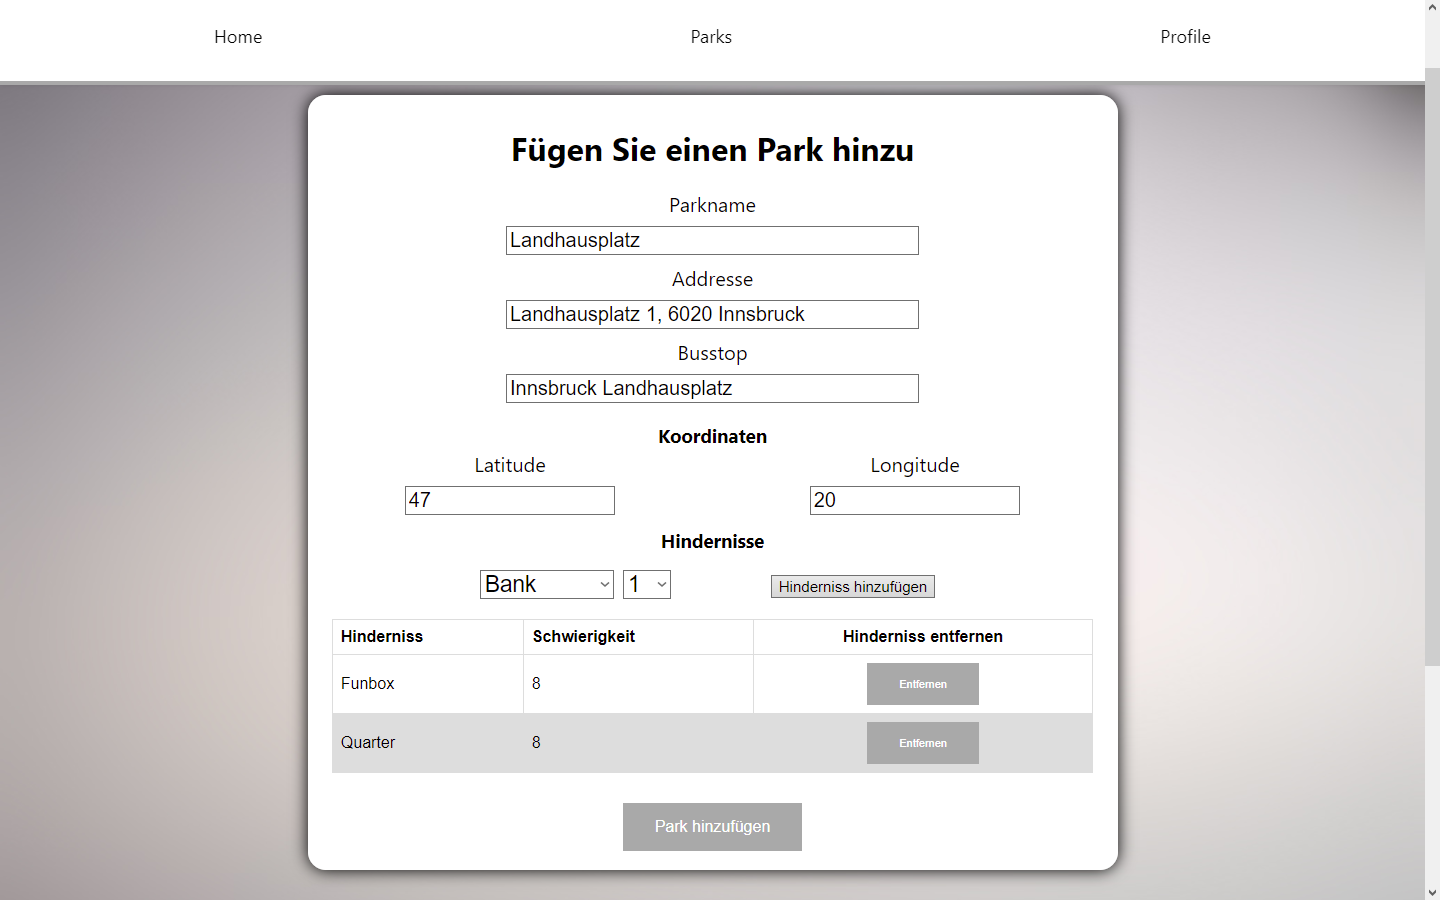
\includegraphics[width=1\textwidth]{Website/Recoom2.png}}
      \caption{Park erstellen}
    \end{center}
\end{figure}

Das Formular zum Park erstellen ist das Selbe wir dies zum Vorschläge erstellen. Benutzt der Admin einen 
Vorschlag welchen man bearbeiten möchte werden die Daten des Vorschlages in die einzelnen Felder 
geladen und können bearbeitet werden. Wurde der Vorschlag fertig bearbeitet und wird als Park der 
Datenbank hinzugefügt, wird der Vorschlag welcher bearbeitet wurde aus der Datenbank gelöscht. 
Wird kein Vorschlag benutzt sonder ein komplett neuer Park erstellt, sind die Input Felder von Anfang 
an leer.
